% D.3 截长补短：△ABC，AD 平分 ∠BAC，AB = AC+CD
\documentclass[tikz,border=4pt]{standalone}
\usepackage{ctex}
\usepackage{amsmath}
\usetikzlibrary{calc}
\begin{document}
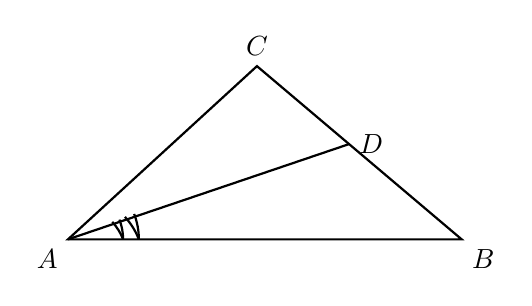
\begin{tikzpicture}[scale=1.0, thick]
  \coordinate (A) at (0, 0);
  \coordinate (B) at (5, 0);
  \coordinate (C) at (2.4, 2.2);
  % D 在 BC 上（AD 平分 ∠BAC）
  \coordinate (D) at ($(B)!0.55!(C)$);

  \draw (A) -- (B) -- (C) -- cycle;
  \draw (A) -- (D);

  % 角弧（标出 AD 平分∠A）
  \draw (0.7,0) arc[start angle=0, end angle=21, radius=0.7];
  \draw (0.9,0) arc[start angle=0, end angle=21, radius=0.9];
  \draw (0.7,0) ++(21:0pt) arc[start angle=21, end angle=42.5, radius=0.7];
  \draw (0.9,0) ++(21:0pt) arc[start angle=21, end angle=42.5, radius=0.9];

  \node[below left]  at (A) {$A$};
  \node[below right] at (B) {$B$};
  \node[above]       at (C) {$C$};
  \node[right]       at (D) {$D$};
\end{tikzpicture}
\end{document}
